\section*{\reportTitle}

La oportunidad del proyecto consiste en ayudar al trabajador a entender su situación antes de iniciar una gestión oficial, con evidencia visible y una derivación pertinente. Dirección del Trabajo (DT), SUSESO y ChileAtiende aportan patrones complementarios: acceso por perfil, preparación y seguimiento, y explicación por necesidad. Las pantallas públicas también muestran fricciones relevantes para las personas UX: jerga, apoyo distante del punto de decisión y acciones cuya prominencia no coincide con la necesidad de comprender primero. El análisis compara experiencias y no determina derechos individuales ni audita legalmente a las instituciones. La propuesta del grupo sigue siendo un concepto: sus capacidades no se presentan como implementadas. Este benchmark fundamenta decisiones para el Customer Journey de Guillermo y para el posterior prototipo.


\section{Tres categorías permiten comparar sin confundir competencias}

La pregunta de investigación es cómo ofrecer orientación comprensible y verificable sobre primera licencia, horas extra impagas y finiquito, sin transformar una explicación en una decisión jurídica. La fecha de consulta es \textbf{5 de octubre de 2026}. Se revisaron fuentes oficiales y nueve capturas públicas, tres por herramienta, obtenidas con un área visible de 866 × 922 píxeles. Esta muestra permite observar páginas, etiquetas, jerarquía y un acordeón abierto; no representa el flujo completo ni todos los dispositivos. Ningún sitio consultado publicó un número de versión en esas páginas; la fecha de actualización de una ficha no equivale a la versión del producto.


El ecosistema bruto considerado comprende DT/Mi DT, SUSESO, ChileAtiende, BCN/Ley Chile y ChatGPT. \textbf{DT es la comparación funcional directa} por su orientación y trámites laborales; SUSESO es un \textbf{análogo sectorial} por preparación, reclamos y seguimiento en seguridad social; ChileAtiende es una \textbf{referencia de diseño de información y derivación}. Se seleccionaron esos tres porque cubren los problemas del repositorio y permiten contrastar interfaces públicas sin asumir que realizan el mismo trabajo. El Centro de Consultas DT organiza temas laborales; SUSESO delimita instituciones y materias fiscalizadas; ChileAtiende comunica beneficios, requisitos y canales. Estas categorías son una decisión metodológica del estudio (\hyperref[ref:ca_descripcion]{ChileAtiende, s. f.-c}; \hyperref[ref:dt_consultas]{Dirección del Trabajo [DT], s. f.-a}; \hyperref[ref:su_competencia]{Superintendencia de Seguridad Social [SUSESO], s. f.-f}).


BCN/Ley Chile se conserva como fuente normativa complementaria, pero se excluye de la matriz principal porque su foco documental no coincide con la preparación y derivación estudiadas; no se inspeccionó su interfaz de consulta. ChatGPT se reconoce como sustituto conversacional general y se excluye de las tres experiencias institucionales por ese alcance distinto. Su documentación reconoce respuestas incorrectas y la necesidad de verificar información: esa limitación refuerza el problema de confianza, pero no constituye una evaluación de su desempeño laboral. La selección no demuestra liderazgo de mercado ni ausencia de alternativas comerciales (\hyperref[ref:bcn]{Biblioteca del Congreso Nacional de Chile [BCN], s. f.}; \hyperref[ref:openai]{OpenAI, s. f.}).


El inventario de la Tabla~\ref{tab:ecosistema} explicita la selección de referentes.

\begin{singlespace}\begin{xltabular}{\textwidth}{@{}p{1.25in}YYY@{}}\caption{Ecosistema considerado y selección de referentes}\label{tab:ecosistema}\\\toprule

\textbf{Nombre} & \textbf{Plataforma y fuente} & \textbf{Clasificación} & \textbf{Selección para la matriz}\\\midrule\endfirsthead

\multicolumn{4}{l}{\textbf{Tabla \thetable} (continuación)}\\\toprule\textbf{Nombre} & \textbf{Plataforma y fuente} & \textbf{Clasificación} & \textbf{Selección para la matriz}\\\midrule\endhead\bottomrule\endfoot\bottomrule\addlinespace[4pt]\multicolumn{4}{@{}p{\linewidth}@{}}{\doublespacing\textit{Nota.} Elaboración del equipo. La categoría es una decisión metodológica, no una clasificación de mercado.}\\\endlastfoot

Dirección del Trabajo / Mi DT & Web institucional y portal de trámites: \hyperref[ref:dt_inicio]{(DT, s. f.-b)} & Comparación funcional directa & Incluida: orientación laboral y preparación de finiquito/horas extra.\\\addlinespace[5pt]

SUSESO & Web institucional y acceso PAE: \hyperref[ref:su_usuarios]{(SUSESO, s. f.-d)} & Análogo sectorial & Incluida: licencia, preparación y seguimiento de reclamos.\\\addlinespace[5pt]

ChileAtiende & Portal web informativo: \hyperref[ref:ca_descripcion]{(ChileAtiende, s. f.-c)} & Referencia de diseño & Incluida: lenguaje cotidiano, acciones y canales.\\\addlinespace[5pt]

BCN / Ley Chile & Aplicación web de consulta normativa: \hyperref[ref:bcn]{(BCN, s. f.)} & Fuente complementaria & Excluida: foco documental; conservar como respaldo normativo.\\\addlinespace[5pt]

ChatGPT & Asistente conversacional web: \hyperref[ref:openai]{(OpenAI, s. f.)} & Sustituto conversacional general & Excluido: alcance distinto de los tres servicios institucionales.\\\addlinespace[5pt]

\end{xltabular}\end{singlespace}

La matriz comparativa aplica diez dimensiones de la pauta —identificación, perfil, valor, funciones priorizadas, onboarding, navegación, diseño, accesibilidad observable, positivos y problemas— y cuatro del dominio: trazabilidad normativa, límites e incertidumbre, derivación competente y privacidad/control. Distingue \textbf{observado}, \textbf{documentado} y \textbf{propuesto}. Las asociaciones con Nielsen interpretan indicios de interfaz; no son resultados de pruebas ni puntajes de severidad medidos. H2 refiere a lenguaje familiar; H3, control; H4, consistencia; H5, prevención de errores; H6, reconocimiento; H8, jerarquía relevante; H10, ayuda contextual (\hyperref[ref:nielsen]{Nielsen, 1994}).


\section{La DT ofrece autoridad, pero el respaldo queda lejos de la decisión}

Las Figuras~\ref{fig:dt01} a~\ref{fig:dt03} documentan la entrada por perfil y dos momentos de la ficha de finiquito.

La DT es pertinente para Guillermo y Joseph: permite consultar derechos laborales y acceder a servicios formales. Las funciones se ordenan aquí por relevancia para esos escenarios: orientación temática, preparación del trámite, acceso a Mi DT y atención humana. \textbf{La lectura pública precede a la autenticación.} La documentación describe RUN y ClaveÚnica para entrar a Mi DT; no se observó la cuenta ni el onboarding interno. Tampoco se fusiona la ruta del empleador con la del trabajador (\hyperref[ref:dt_perfiles]{DT, 2022}; \hyperref[ref:dt_ingreso]{DT, 2023}).


En DT01, las tarjetas de trabajadores y empleadores constituyen un primer positivo: hacen reconocible el perfil pertinente (H6). En DT03, un segundo positivo es la presencia de ayuda por SUAC y teléfono junto con un enlace al marco legal: ofrece apoyo verificable (H10). Sin embargo, el aviso sobre Clave Tributaria del gestor de representantes laborales ocupa la parte superior de DT01, antes de la entrada del trabajador. Para el objetivo de orientación de Joseph, esa prioridad introduce información de otro perfil (H8). En DT02–DT03, la extensión de la ficha y el respaldo legal al final obligan a recorrer contenido y relacionarlo con la explicación inicial (H6/H8). Son problemas potenciales de localización, no evidencia de abandono (\hyperref[ref:dt_inicio]{DT, s. f.-b}; \hyperref[ref:dt_finiquito]{DT, s. f.-c}).


La ficha explica modalidades y documentos, pero términos como “ministro de fe” permanecen sin glosario en el fragmento observado; el manual externo amplía instrucciones sin sustituir una ayuda breve en contexto. Visualmente predominan azul institucional, tarjetas grandes y títulos de sección. Los controles de tamaño de texto son visibles, y DT01 muestra desplazamiento horizontal: ninguno de estos indicios acredita accesibilidad completa. El recorrido público observado fue portada → \hyperref[ref:dt_trabajadores]{(DT, s. f.-d)} → ficha de finiquito: tres páginas. Las capturas muestran portada y ficha arriba/abajo; la profundidad transaccional de Mi DT queda desconocida (\hyperref[ref:dt_finiquito]{DT, s. f.-c}).


\clearpage\begin{figure}[p]\centering
\caption{Entrada por perfiles y aviso previo en la DT}\label{fig:dt01}
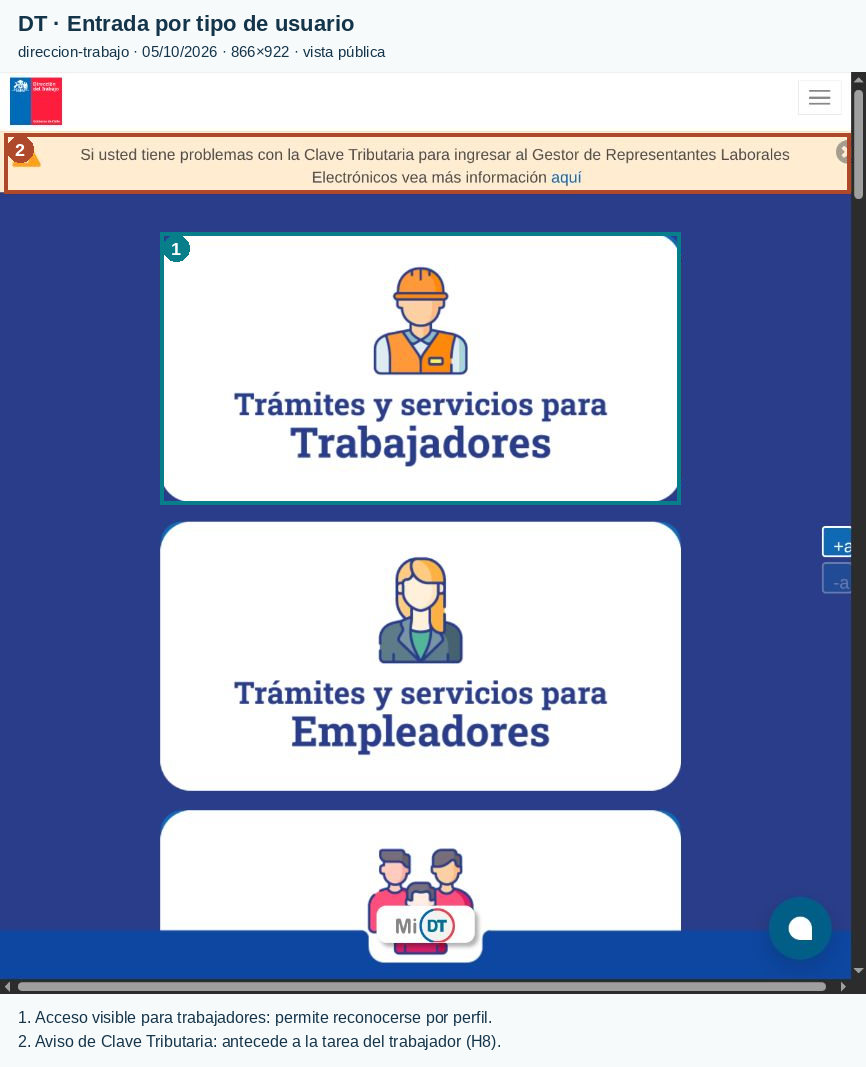
\includegraphics[width=\textwidth,height=0.70\textheight,keepaspectratio]{../capturas/direccion-trabajo/01-anotada.png}
\par\smallskip\begin{figurenote}\textit{Nota.} Perfiles reconocibles; el aviso de representantes laborales antecede la entrada del trabajador. Captura y anotaciones del equipo sobre DT (s. f.-b); observación del 5 de octubre de 2026.\end{figurenote}\end{figure}\clearpage

\clearpage\begin{figure}[p]\centering
\caption{Descripción y requisitos del finiquito en la DT}\label{fig:dt02}
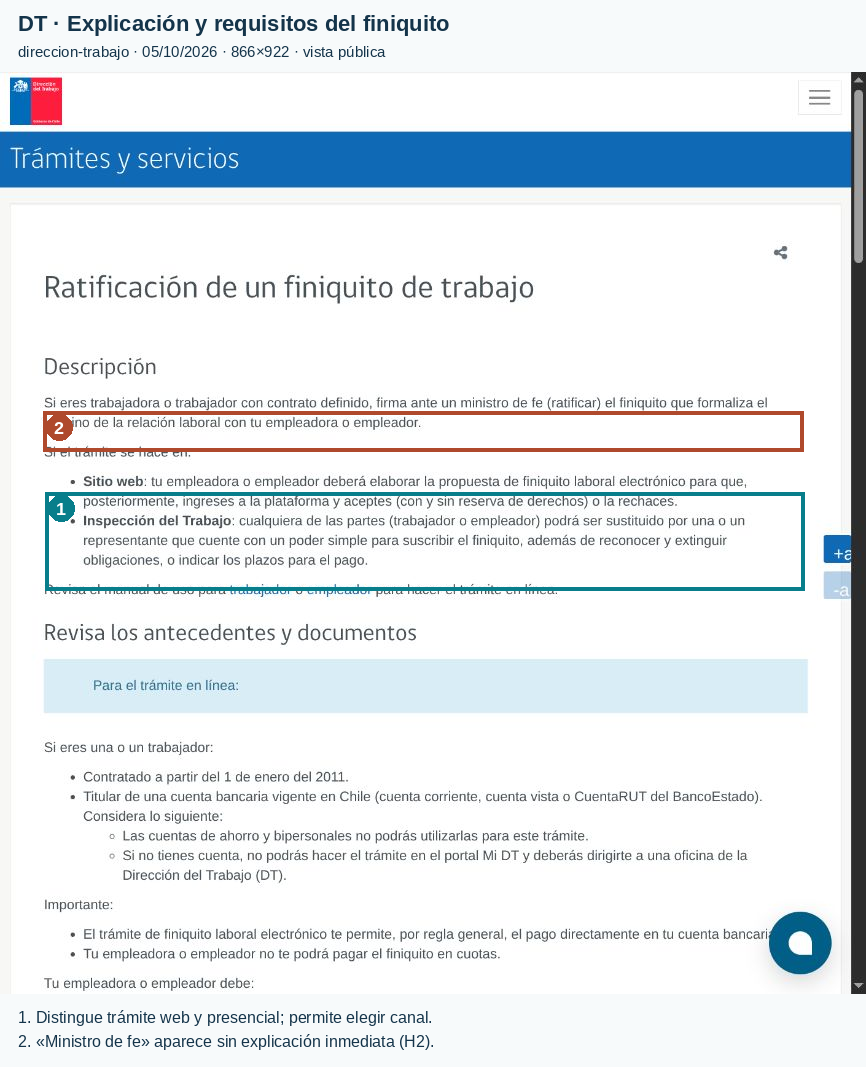
\includegraphics[width=\textwidth,height=0.70\textheight,keepaspectratio]{../capturas/direccion-trabajo/02-anotada.png}
\par\smallskip\begin{figurenote}\textit{Nota.} Descripción y documentos; el manual externo no reemplaza un glosario breve en contexto. Captura y anotaciones del equipo sobre DT (s. f.-c); observación del 5 de octubre de 2026.\end{figurenote}\end{figure}\clearpage

\clearpage\begin{figure}[p]\centering
\caption{Ayuda y respaldo legal al final de la ficha de la DT}\label{fig:dt03}
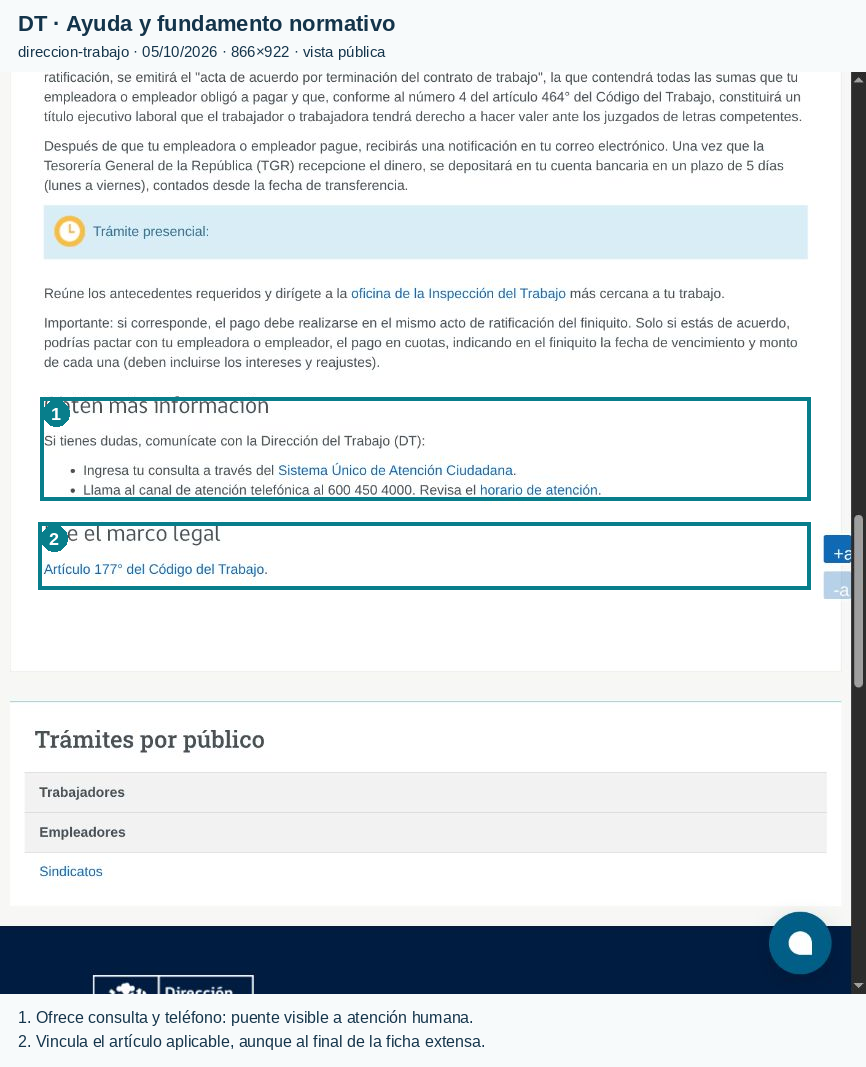
\includegraphics[width=\textwidth,height=0.70\textheight,keepaspectratio]{../capturas/direccion-trabajo/03-anotada.png}
\par\smallskip\begin{figurenote}\textit{Nota.} Ayuda y fundamento disponibles al final de una ficha extensa. Captura y anotaciones del equipo sobre DT (s. f.-c); observación del 5 de octubre de 2026.\end{figurenote}\end{figure}\clearpage

\section{SUSESO separa intenciones, aunque exige reconocer lenguaje institucional}

Las Figuras~\ref{fig:su01} a~\ref{fig:su03} muestran el acceso, la selección por perfil y la clasificación del problema.

SUSESO resulta especialmente pertinente para Benjamin por sus servicios de seguridad social. El orden funcional relevante es orientación, preparación de antecedentes, simulación estimada del subsidio, reclamo y seguimiento. En SU01 se distinguen “Reclamos” y “Seguimiento del reclamo”: \textbf{primer positivo, acciones reconocibles} sin confundir iniciar y consultar (H6). SU02 selecciona orientación para trabajadores, familias u otras necesidades: segundo positivo, clasificación por perfil y situación (H2/H6). No se inspeccionó un expediente real ni se midió cuánto tarda una persona en elegir (\hyperref[ref:su_orientador]{SUSESO, s. f.-c}; \hyperref[ref:su_usuarios]{SUSESO, s. f.-d}).


El tramo observado permite describir orientador → trabajadores → licencias → dos situaciones. SU03 presenta rechazo/modificación y ausencia de pronunciamiento de COMPIN. Para una primera licencia, “pronunciada” y la sigla institucional requieren conocimiento previo sin definición visible en ese fragmento: \textbf{primer problema, jerga} (H2). Además, el control lateral de tamaño de texto tapa parcialmente “Volver” en el área capturada: segundo problema, interferencia con la salida (H3/H8). La interfaz muestra opciones grandes y contraste aparente azul/blanco, pero el contraste no fue medido. La superposición corresponde a ese tamaño de ventana; no se generaliza a todos los dispositivos (\hyperref[ref:su_licencias]{SUSESO, s. f.-b}).


El contenido público del simulador declara que su resultado es estimado y delimita qué casos considera. Ese patrón es transferible: explicar supuestos antes de entregar una cifra. El ciclo publicado documenta preparación, revisión y consulta de estados, pero no demuestra que las pantallas privadas actuales coincidan exactamente con el tutorial. La pantalla de ingreso ofrece ClaveÚnica y Clave Tributaria; una mención histórica a crear contraseña no se toma como alternativa personal vigente (\hyperref[ref:su_ciclo]{SUSESO, s. f.-a}; \hyperref[ref:su_pae]{SUSESO, s. f.-e}; \hyperref[ref:su_simulador]{SUSESO, s. f.-i}).


\clearpage\begin{figure}[p]\centering
\caption{Reclamos y seguimiento separados en SUSESO}\label{fig:su01}
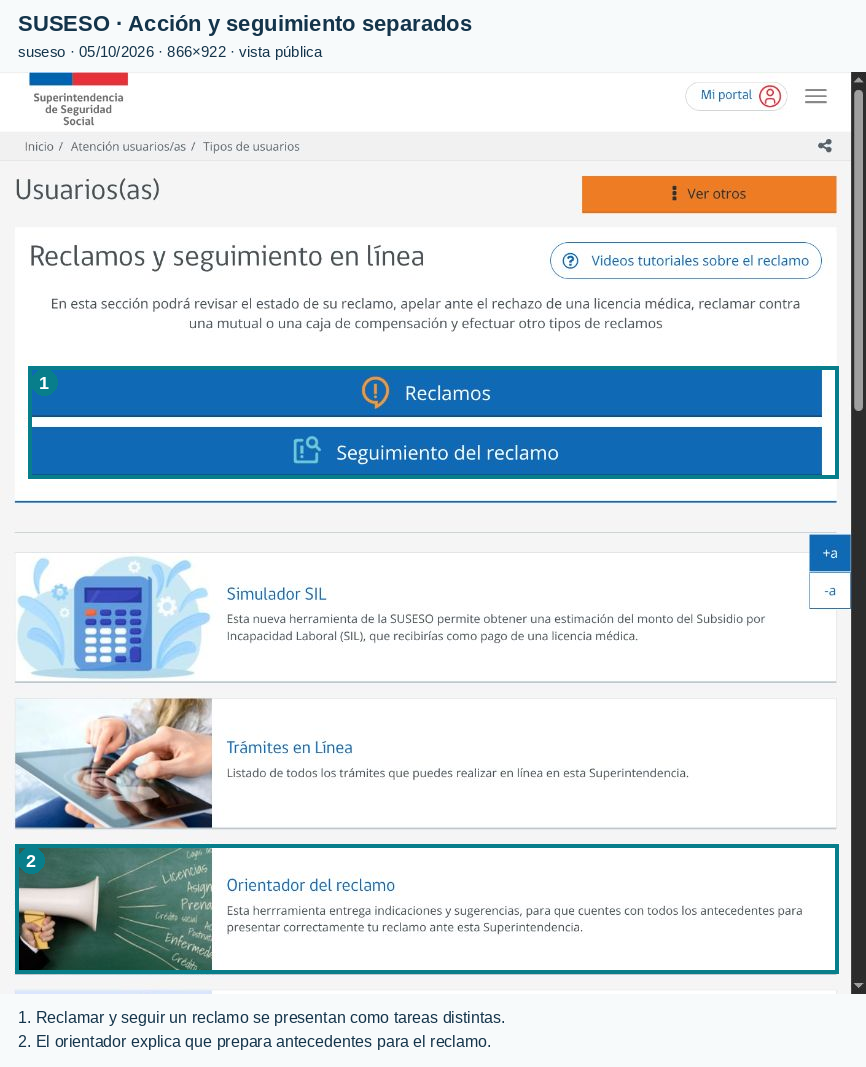
\includegraphics[width=\textwidth,height=0.70\textheight,keepaspectratio]{../capturas/suseso/01-anotada.png}
\par\smallskip\begin{figurenote}\textit{Nota.} Iniciar y seguir un reclamo son acciones distintas; el simulador se presenta como estimación. Captura y anotaciones del equipo sobre SUSESO (s. f.-d); observación del 5 de octubre de 2026.\end{figurenote}\end{figure}\clearpage

\clearpage\begin{figure}[p]\centering
\caption{Orientación por perfiles en SUSESO}\label{fig:su02}
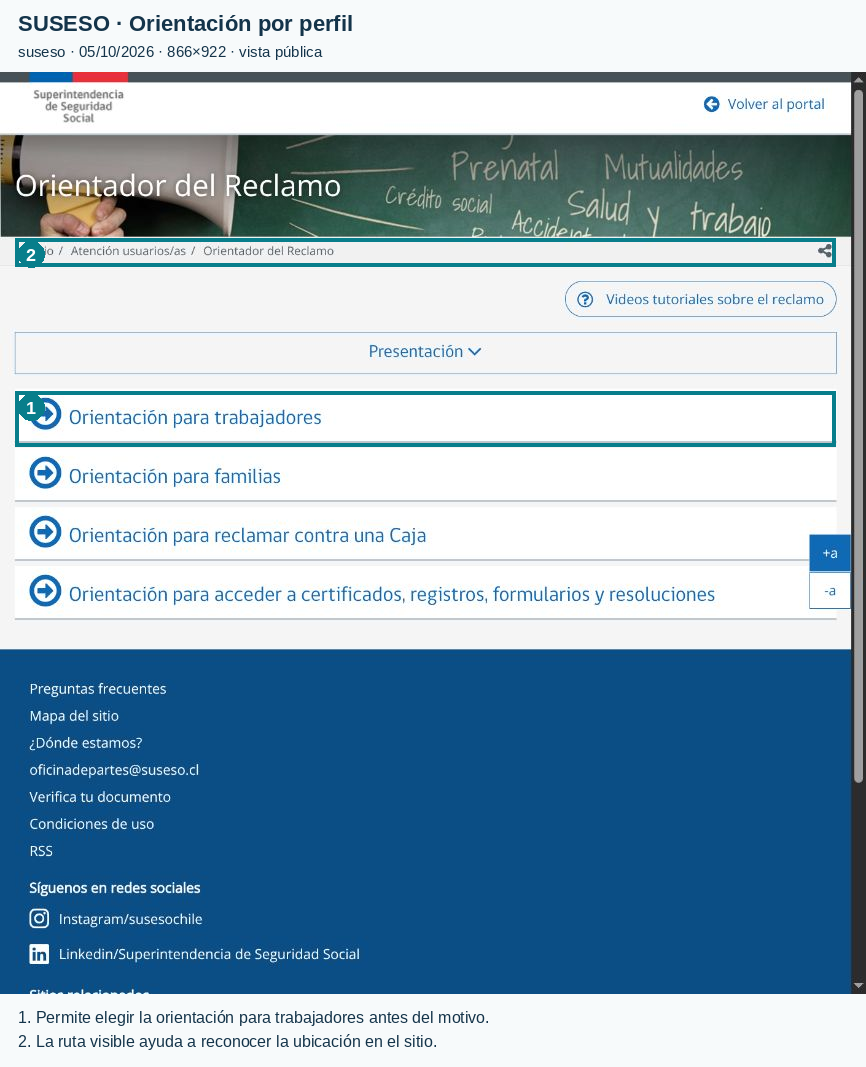
\includegraphics[width=\textwidth,height=0.70\textheight,keepaspectratio]{../capturas/suseso/02-anotada.png}
\par\smallskip\begin{figurenote}\textit{Nota.} La selección por perfil prepara la ruta antes de pedir autenticación. Captura y anotaciones del equipo sobre SUSESO (s. f.-c); observación del 5 de octubre de 2026.\end{figurenote}\end{figure}\clearpage

\clearpage\begin{figure}[p]\centering
\caption{Lenguaje institucional y control superpuesto en SUSESO}\label{fig:su03}
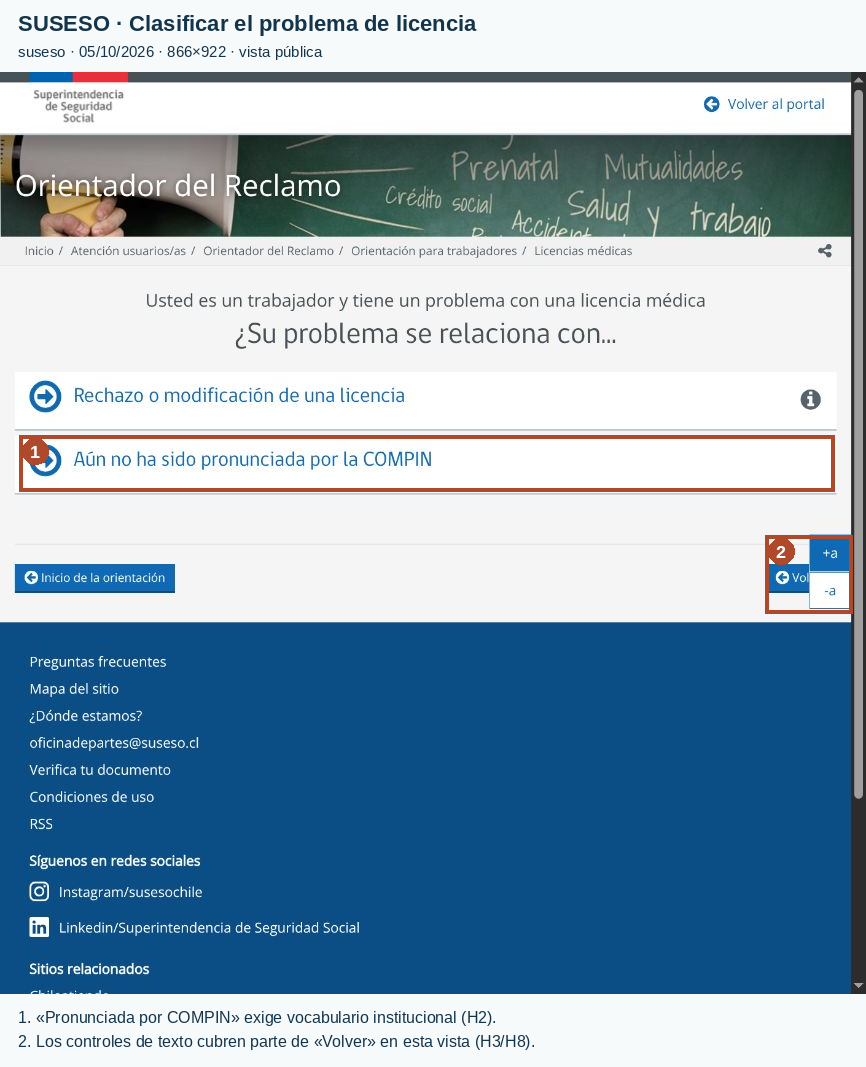
\includegraphics[width=\textwidth,height=0.70\textheight,keepaspectratio]{../capturas/suseso/03-anotada.png}
\par\smallskip\begin{figurenote}\textit{Nota.} Lenguaje institucional y superposición parcial de “Volver” en el tamaño observado. Captura y anotaciones del equipo sobre SUSESO (s. f.-b); observación del 5 de octubre de 2026.\end{figurenote}\end{figure}\clearpage

\section{ChileAtiende explica por acciones y necesita equilibrar ayuda y trámite}

Las Figuras~\ref{fig:ca01} a~\ref{fig:ca03} registran explicación, opciones de ratificación y canales de atención.

ChileAtiende funciona como referencia de información, no como autoridad que resuelve el caso laboral. Ordenamos sus capacidades por relevancia: explicación de la necesidad, requisitos y pasos, derivación a la institución responsable y selección del canal. La ficha de Joseph permite observar lectura pública → sección de ratificación abierta → enlace externo a DT o alternativa presencial; no se completó el trámite. La fecha \textbf{27 de enero de 2026} aparece como última actualización de esa ficha (\hyperref[ref:ca_finiquito]{ChileAtiende, 2026}).


Un primer positivo en CA01 es la aclaración “causal (motivo)”: traduce un término especializado (H2). Un segundo positivo en CA02 son las acciones separadas “Obtén” y “Ratifica”, con información desplegable y destinos explícitos (H6/H8). La asesoría gratuita está enlazada en la descripción. No obstante, la barra fija destaca “Ratificar finiquito” por encima de “Ayuda”; para Joseph, que busca comprender antes de actuar, esa jerarquía merece revisión (H8). El problema no es la existencia del botón sino su prioridad respecto del objetivo del escenario (\hyperref[ref:ca_finiquito]{ChileAtiende, 2026}).


CA03 muestra canales remotos y presenciales mediante tarjetas explicativas. Entre ficha y red de atención cambian cabecera y tratamiento tipográfico: \textbf{segundo problema, consistencia visual} (H4). Las redes sociales anteceden a canales de atención, una prioridad adicional poco alineada con una necesidad urgente (H8). Los enlaces subrayados y el contorno visible del acordeón ayudan a reconocer interacción; no se comprobaron teclado ni lector de pantalla. El portal no debe recibir crédito por resolver, cargar documentos o calcular finiquitos: las fichas derivan al servicio responsable (\hyperref[ref:ca_red]{ChileAtiende, s. f.-d}).


\clearpage\begin{figure}[p]\centering
\caption{Explicación del finiquito y acción fija en ChileAtiende}\label{fig:ca01}
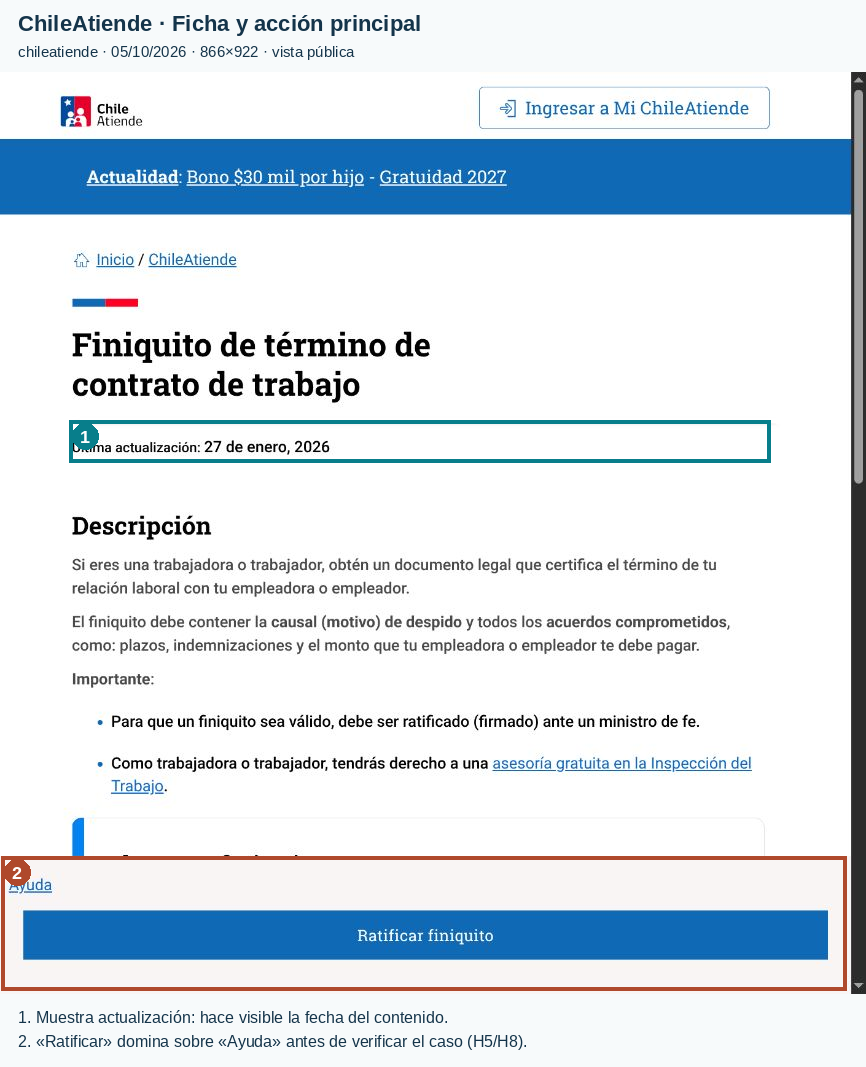
\includegraphics[width=\textwidth,height=0.70\textheight,keepaspectratio]{../capturas/chileatiende/01-anotada.png}
\par\smallskip\begin{figurenote}\textit{Nota.} Traducción de términos y fecha visibles; ratificar domina visualmente a la ayuda. Captura y anotaciones del equipo sobre ChileAtiende (2026); observación del 5 de octubre de 2026.\end{figurenote}\end{figure}\clearpage

\clearpage\begin{figure}[p]\centering
\caption{Alternativas de ratificación en ChileAtiende}\label{fig:ca02}
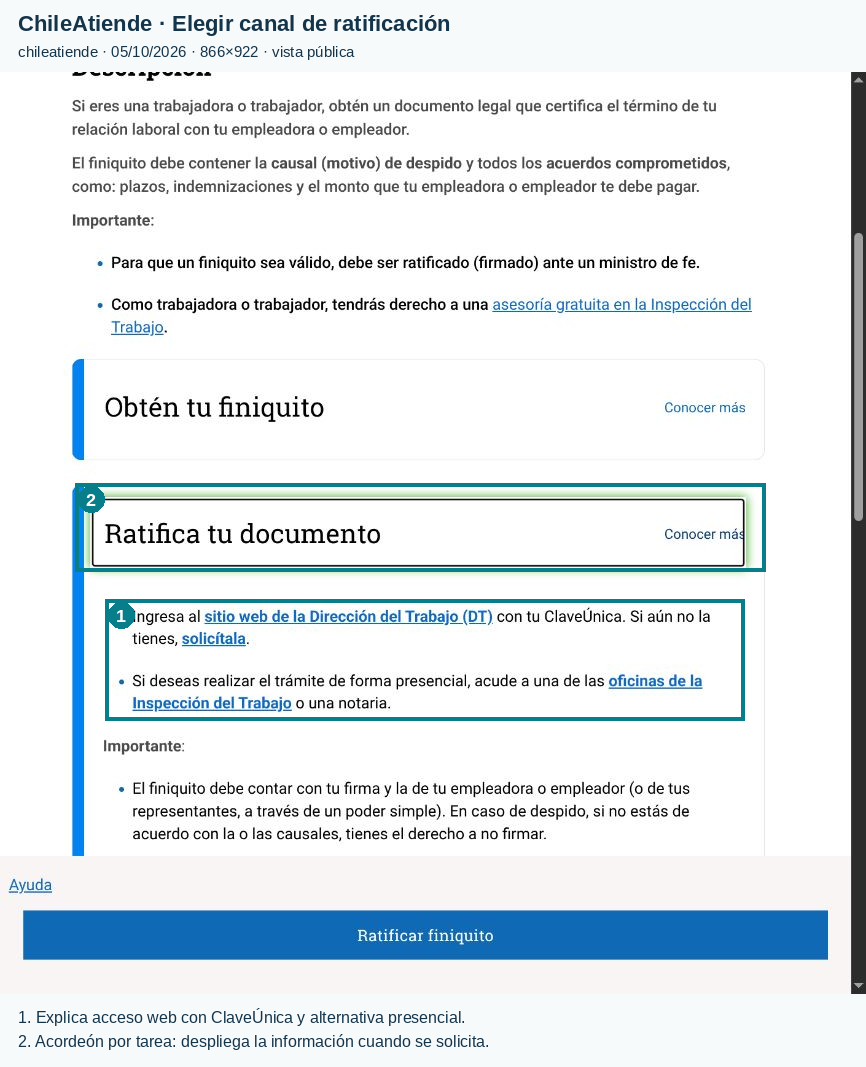
\includegraphics[width=\textwidth,height=0.70\textheight,keepaspectratio]{../capturas/chileatiende/02-anotada.png}
\par\smallskip\begin{figurenote}\textit{Nota.} La sección abierta identifica DT, ClaveÚnica y alternativa presencial. Captura y anotaciones del equipo sobre ChileAtiende (2026); observación del 5 de octubre de 2026.\end{figurenote}\end{figure}\clearpage

\clearpage\begin{figure}[p]\centering
\caption{Canales de la red de atención de ChileAtiende}\label{fig:ca03}
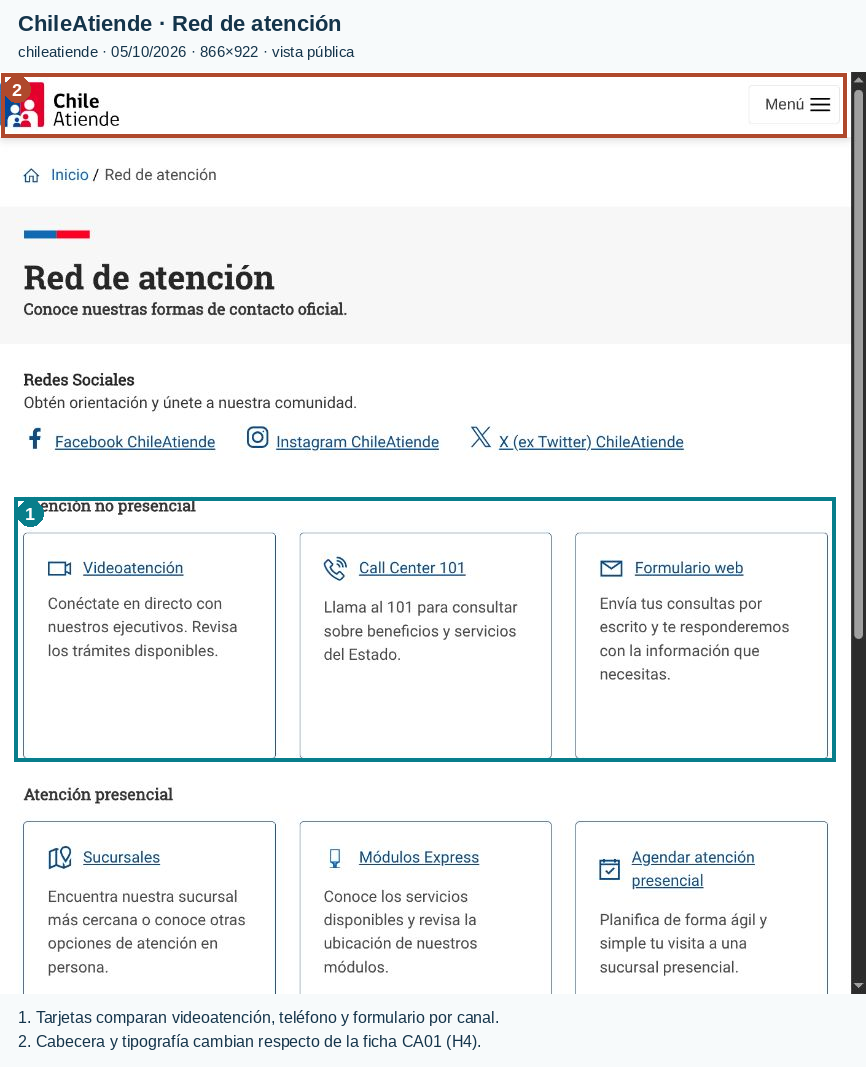
\includegraphics[width=\textwidth,height=0.70\textheight,keepaspectratio]{../capturas/chileatiende/03-anotada.png}
\par\smallskip\begin{figurenote}\textit{Nota.} Canales explicados; redes sociales primero y tratamiento visual distinto de la ficha. Captura y anotaciones del equipo sobre ChileAtiende (s. f.-d); observación del 5 de octubre de 2026.\end{figurenote}\end{figure}\clearpage

\section{El prototipo debe priorizar comprensión, evidencia y control}

\textbf{Garrett: Estrategia.} El modelo de \hyperref[ref:garrett]{Garrett (2011)} relaciona necesidades de usuarios y objetivos del producto. La necesidad que guía el concepto es comprender con respaldo antes de actuar; su objetivo de producto es orientar hacia la instancia pertinente con confianza explicada. Las prioridades siguientes son \textbf{propuestas para validación del equipo, no decisiones aprobadas}. Los hallazgos refinan el Canvas de propuesta de valor y las personas UX. Para Benjamin, proponemos adoptar el acceso por situación y la preparación progresiva de SUSESO, rechazando comenzar con jerga o un reclamo prematuro. Para Guillermo, proponemos adoptar fuentes oficiales y apoyo humano de DT, rechazando pedir identificación al iniciar una orientación general o prometer ausencia de represalias. Su ocupación no basta para determinar el régimen de jornada: corresponde preguntar el tipo de transporte y registros disponibles antes de orientar. Para Joseph, proponemos adoptar explicación cotidiana y alternativas de ChileAtiende, rechazando dar más prominencia a firmar que a comprender. Estas son \textbf{hipótesis de diseño}, no preferencias comprobadas con las personas (\hyperref[ref:dt_jornada]{DT, 2024}).


\textbf{Garrett: Alcance.} El mismo modelo ayuda a delimitar las capacidades y los requisitos de contenido. Proponemos priorizar un recorrido acotado en el prototipo: seleccionar el problema, reunir contexto mínimo, explicar con fuente y fecha de revisión, mostrar qué falta para responder y preparar una derivación. Proponemos que la fuente acompañe la afirmación, en lugar de quedar al final de un documento. El nivel de confianza propuesto en el Canvas se expresará mediante razones comprensibles —fuente pertinente, antecedentes faltantes o discrepancias—, sin porcentajes arbitrarios ni una etiqueta que prometa certeza jurídica. El mapa de capacidades resume lo observado, lo documentado y lo que se propone ensayar.


La Figura~\ref{fig:mapa} integra capacidades observadas, documentadas y propuestas.

\clearpage\begin{figure}[p]\centering
\caption{Mapa comparativo de capacidades y oportunidades de diseño}\label{fig:mapa}
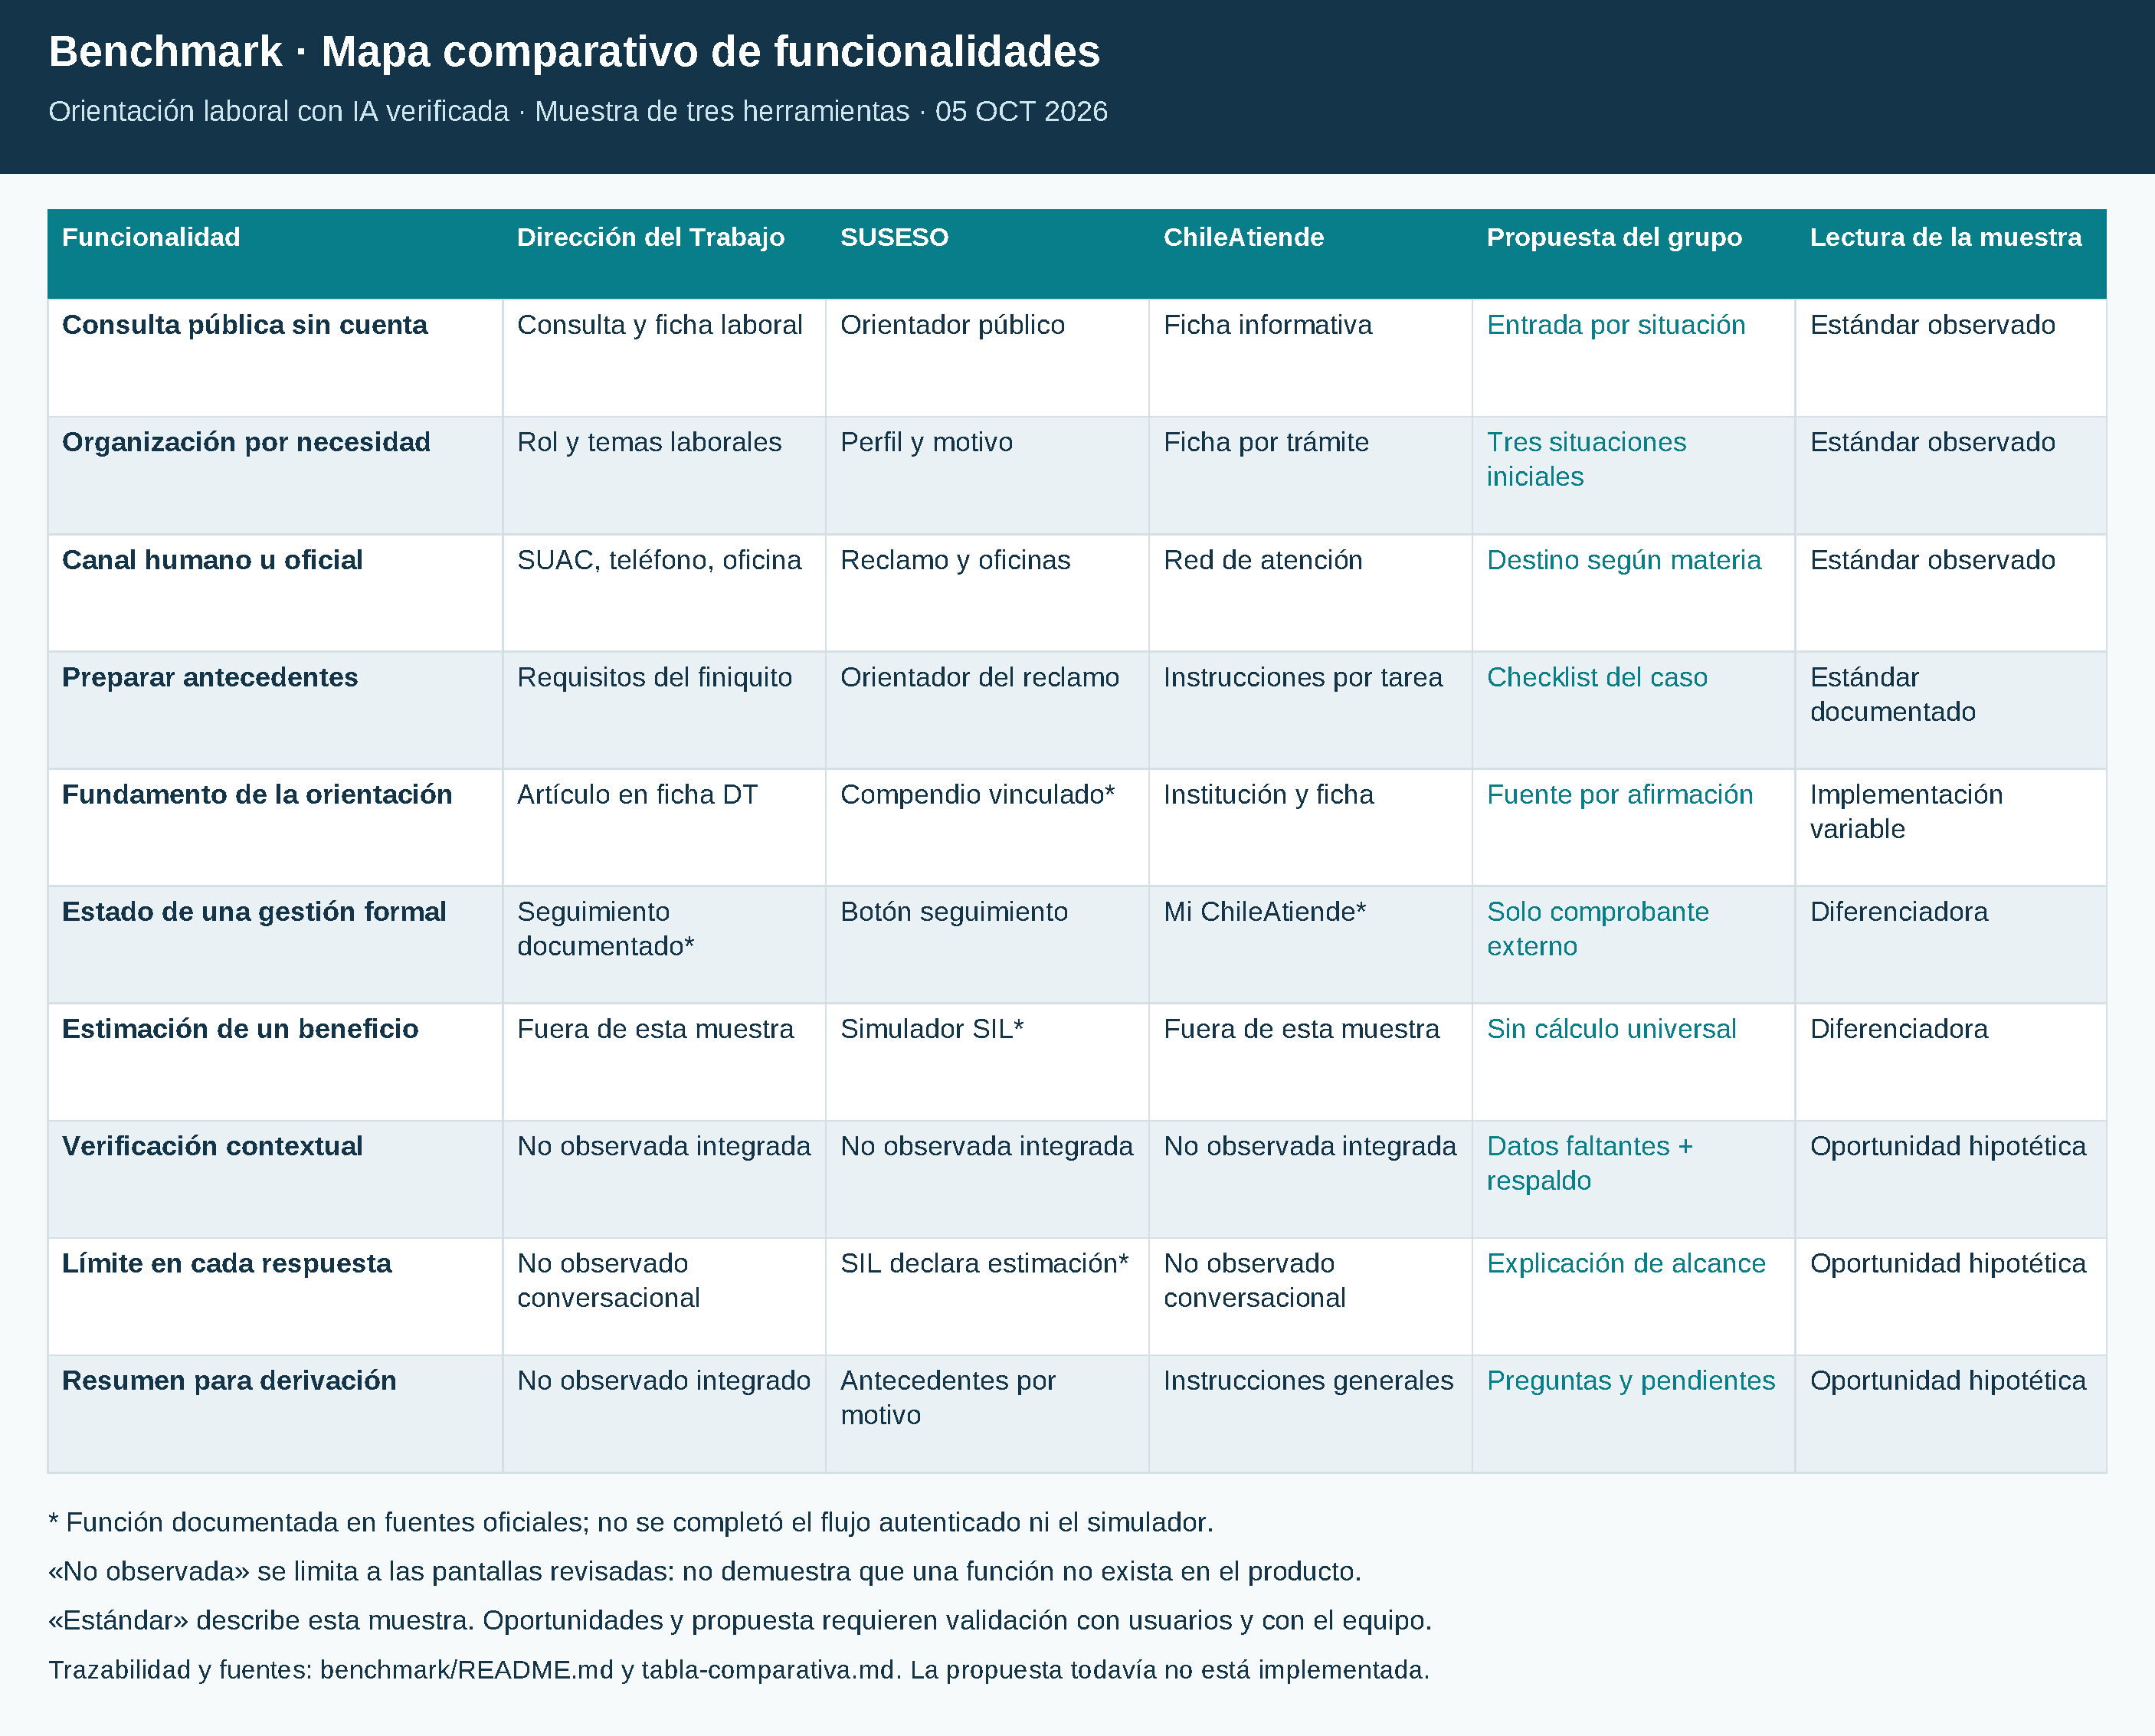
\includegraphics[width=\textwidth,keepaspectratio]{../feature-map.pdf}
\par\smallskip\begin{figurenote}\textit{Nota.} Elaboración del equipo a partir del benchmark; las capacidades documentadas no equivalen a pruebas ejecutadas. La propuesta del grupo es una hipótesis.\end{figurenote}\end{figure}\clearpage

Una segunda prioridad es continuidad: resumen revisable, checklist de documentos y alternativa de orientación humana. Se propone guardar información únicamente por decisión explícita del usuario, explicar su uso y permitir eliminarla; \textbf{no se verificaron políticas de retención ni controles de borrado} de los tres referentes. La lectura pública demuestra que es posible ofrecer información sin iniciar sesión, pero no prueba ausencia de rastreo. El benchmark no recomienda recolectar antecedentes médicos para explicar una primera licencia ni almacenar documentos laborales en la primera versión.


El Canvas plantea derivación automática a la Inspección del Trabajo ante casos complejos. La investigación exige refinar ese destino: \textbf{la derivación depende de materia y etapa}. DT orienta asuntos laborales, mientras las rutas de licencias pueden requerir COMPIN o SUSESO. No se convierte una discrepancia entre resúmenes oficiales en una instrucción individual; se muestra el límite y se verifica la fuente competente. Se excluyen del alcance inicial firma o envío de trámites, cálculo definitivo de indemnizaciones, diagnóstico médico, pronunciamiento sobre legalidad y garantías de éxito de reclamos (\hyperref[ref:dt_licencias]{DT, 2025}; \hyperref[ref:su_compendio]{SUSESO, s. f.-h}).


\section{La siguiente evidencia debe comprobar comprensión antes de acción}

\textbf{El estado es fase 2 documental con inspección de interfaz pública.} Quedan pendientes el uso supervisado de flujos autenticados, la comprobación de accesibilidad y la validación grupal del diagnóstico y las prioridades. No se atribuye esta revisión a reuniones, entrevistas, reseñas o pruebas que no ocurrieron. Para avanzar, el equipo debe acordar escenarios equivalentes por persona y observar si participantes pueden explicar su situación, localizar el respaldo y escoger una ayuda pertinente sin confundir orientación con resolución oficial.


El Customer Journey de Guillermo traduce estas hipótesis a puntos de contacto y oportunidades; sus emociones deben identificarse como inferidas. La evaluación posterior necesita observar especialmente tres errores: Benjamin inicia una reclamación que no corresponde a su etapa; Guillermo aplica una regla de jornada sin clasificar su trabajo; Joseph interpreta una respuesta como autorización para firmar. Reducir esas confusiones es un criterio más útil para este proyecto que contar funciones o declarar ganador a un portal con otro mandato.


\clearpage\section{Matriz comparativa}

Las Tablas~\ref{tab:matrix1} a~\ref{tab:matrix4} desarrollan diez dimensiones base y cuatro del dominio. Cada tabla incluye la propuesta del grupo como fila completa. O significa observado en nueve capturas públicas; D, documentado en fuentes oficiales; y P, propuesta para validar. Las prioridades expresan pertinencia para las personas, sin frecuencia de uso medida.


No se calcula un puntaje global: las herramientas cumplen mandatos distintos y la propuesta aún no es un producto evaluado. La matriz complementa los análisis y las Figuras~\ref{fig:dt01} a~\ref{fig:mapa}.


\clearpage\begin{landscape}\begin{singlespace}\fontsize{10}{11}\selectfont\setlength{\tabcolsep}{5pt}\begin{xltabular}{\linewidth}{@{}p{1.02in}YYYYY@{}}

\caption{Identificación, usuarios y capacidades}\label{tab:matrix1}\\\toprule

\textbf{Herramienta} & \textbf{Categoría y pertinencia} & \textbf{1. Identificación, plataforma, fecha y versión} & \textbf{2. Perfil y escenario de uso} & \textbf{3. Propuesta de valor} & \textbf{4. Funcionalidades ordenadas por relevancia}\\\midrule\endfirsthead

\multicolumn{6}{l}{\textbf{Tabla \thetable} (continuación)}\\\toprule\textbf{Herramienta} & \textbf{Categoría y pertinencia} & \textbf{1. Identificación, plataforma, fecha y versión} & \textbf{2. Perfil y escenario de uso} & \textbf{3. Propuesta de valor} & \textbf{4. Funcionalidades ordenadas por relevancia}\\\midrule\endhead\bottomrule\endfoot\bottomrule\addlinespace[4pt]\multicolumn{6}{@{}p{\linewidth}@{}}{\doublespacing\normalsize\textit{Nota.} Elaboración del equipo; observación del 5 de octubre de 2026. O = observado; D = documentado; P = propuesto. Las citas remiten a las referencias del informe.}\\\endlastfoot

Dirección del Trabajo / Mi DT & Comparación funcional directa: orientación y servicios laborales; especialmente horas extra y finiquito. & Web institucional y portal Mi DT. Consulta 05/10/2026; versión no publicada en páginas revisadas. D: FAQ de acceso modificada 14/12/2023, sin equivaler a versión actual. \hyperref[ref:dt_ingreso]{(DT, 2023)}. & O: entradas trabajadores/empleadores/sindicatos. D: orientación de jornada para Guillermo y ficha finiquito para Joseph; régimen de transporte exige contexto. \hyperref[ref:dt_jornada]{(DT, 2024)}. & D: orientación laboral, acceso a gestión formal y canales de ayuda institucionales. \hyperref[ref:dt_consultas]{(DT, s. f.-a)}. & 1 D: consultas temáticas; 2 O: requisitos/documentos del finiquito; 3 D: Mi DT; 4 O: SUAC/teléfono/presencial. \hyperref[ref:dt_finiquito]{(DT, s. f.-c)}.\\\addlinespace[3pt]

SUSESO & Análogo sectorial: seguridad social, preparación y seguimiento; especialmente licencia de Benjamin. & Web institucional y PAE. Consulta 05/10/2026; versión no publicada en páginas revisadas. \hyperref[ref:su_usuarios]{(SUSESO, s. f.-d)}. & O: trabajadores, familias y otros perfiles; licencias de Benjamin. La competencia de seguridad social no convierte al portal en solución de finiquito. \hyperref[ref:su_orientador]{(SUSESO, s. f.-c)}. & D: orientar, tramitar y resolver reclamos de seguridad social relativos a entidades fiscalizadas. \hyperref[ref:su_competencia]{(SUSESO, s. f.-f)}. & 1 O: orientador; 2 D: preparación; 3 D: estimación SIL; 4 O: acceso a reclamo; 5 O: entrada de seguimiento, sin expediente observado. \hyperref[ref:su_ciclo]{(SUSESO, s. f.-a)}, \hyperref[ref:su_simulador]{(SUSESO, s. f.-i)}.\\\addlinespace[3pt]

ChileAtiende & Referencia de información y derivación multiservicios; especialmente comprensión de Joseph y selección de canales. & Web institucional administrada por IPS. Consulta 05/10/2026; versión no publicada; O: ficha finiquito actualizada 27/01/2026. \hyperref[ref:ca_finiquito]{(ChileAtiende, 2026)}. & D: personas que necesitan beneficios o trámites del Estado; O: ficha para trabajador que recibe finiquito y alternativas de atención. \hyperref[ref:ca_descripcion]{(ChileAtiende, s. f.-c)}. & D: explicar requisitos y cómo/dónde realizar trámites; derivar a instituciones responsables. \hyperref[ref:ca_descripcion]{(ChileAtiende, s. f.-c)}. & 1 O: explicación; 2 O: pasos desplegables; 3 O: enlaces DT/presencial; 4 O: red de canales. No se observó cálculo individual ni carga documental. \hyperref[ref:ca_red]{(ChileAtiende, s. f.-d)}.\\\addlinespace[3pt]

Propuesta del grupo & P: orientación laboral asistida por IA con evidencia; puente entre comprender y acudir al organismo pertinente. & P: concepto del curso; no existe versión de producto implementado. Benchmark documental y público de 05/10/2026. & P: Benjamin (primera licencia), Guillermo (horas impagas) y Joseph (finiquito); entradas por problema cotidiano y contexto mínimo. & P: entender antes de actuar; explicación simple con respaldo, límites y próxima acción pertinente, sin sustituir decisión oficial. & P: 1 clasificar situación; 2 responder con evidencia; 3 exponer datos faltantes; 4 checklist/derivación; 5 resumen guardable por elección.\\\addlinespace[3pt]

\end{xltabular}\end{singlespace}\end{landscape}

\clearpage\begin{landscape}\begin{singlespace}\fontsize{10}{12}\selectfont\setlength{\tabcolsep}{5pt}\begin{xltabular}{\linewidth}{@{}p{1.02in}YYYY@{}}

\caption{Acceso, navegación e interfaz}\label{tab:matrix2}\\\toprule

\textbf{Herramienta} & \textbf{5. Onboarding: público frente a documentado} & \textbf{6. Navegación y profundidad observada} & \textbf{7. Diseño visual e interacción} & \textbf{8. Accesibilidad observable}\\\midrule\endfirsthead

\multicolumn{5}{l}{\textbf{Tabla \thetable} (continuación)}\\\toprule\textbf{Herramienta} & \textbf{5. Onboarding: público frente a documentado} & \textbf{6. Navegación y profundidad observada} & \textbf{7. Diseño visual e interacción} & \textbf{8. Accesibilidad observable}\\\midrule\endhead\bottomrule\endfoot\bottomrule\addlinespace[4pt]\multicolumn{5}{@{}p{\linewidth}@{}}{\doublespacing\normalsize\textit{Nota.} Elaboración del equipo; observación del 5 de octubre de 2026. O = observado; D = documentado; P = propuesto. Las citas remiten a las referencias del informe.}\\\endlastfoot

Dirección del Trabajo / Mi DT & O: portada y ficha legibles sin cuenta. D: Mi DT requiere RUN/ClaveÚnica; no se inspeccionó la sesión. \hyperref[ref:dt_ingreso]{(DT, 2023)}. & O: portada → Trabajadores → ficha de finiquito; recorrido de tres páginas públicas, con secciones verticales. Soporte/marco legal al final. Capturas de portada y ficha arriba/abajo; Mi DT privado no observado. \hyperref[ref:dt_trabajadores]{(DT, s. f.-d)}. & O: azul institucional, tarjetas grandes, títulos y párrafos/listas; manual externo. Aviso ocupa franja superior. & O: controles +a/−a y títulos; DT01 tiene desplazamiento horizontal. No se midieron contraste, semántica, zoom ni teclado.\\\addlinespace[7pt]

SUSESO & O: selección y orientación pública. D: PAE ofrece ClaveÚnica/Tributaria y contraseña para personas jurídicas; no se ingresó ni se validó un tutorial antiguo de contraseña personal. \hyperref[ref:su_pae]{(SUSESO, s. f.-e)}. & O: usuarios y orientador; tramo orientador → trabajadores → licencias → dos situaciones. No se observó el final de cada rama ni profundidad autenticada. & O: azul/blanco, botones amplios, imágenes por servicio, migas de navegación y retorno. & O: controles +a/−a; en SU03 tapan parcialmente Volver al tamaño de captura. No hay auditoría WCAG ni prueba con lector.\\\addlinespace[7pt]

ChileAtiende & O: ficha y acordeón públicos. D: ratificación en DT con ClaveÚnica; la cuenta del portal no fue inspeccionada. \hyperref[ref:ca_finiquito]{(ChileAtiende, 2026)}. & O: ficha → acordeón Ratifica abierto; red de atención en otra página. El enlace a DT es visible; gestión en destino no ejecutada. & O: título, fecha y acordeones; acción fija de ratificación; red de atención usa tarjetas y cabecera distinta. & O: enlaces subrayados y contorno visible del acordeón abierto. Sin prueba de teclado, zoom, lector o contraste.\\\addlinespace[7pt]

Propuesta del grupo & P: orientación inicial sin cuenta; explicar por qué se solicita cada dato; autenticación institucional sólo en el destino competente. & P: situación → preguntas mínimas → respuesta/alcance → revisar checklist → elegir canal. Retroceso y edición disponibles en el prototipo. & P: jerarquía comprensión → evidencia → acción; componentes consistentes, fuente al lado de la afirmación, ayuda breve en contexto. & P: lenguaje simple, controles que no se superpongan, foco visible y contraste verificable. Evaluar teclado, zoom y lector en prototipo; no declarar conformidad anticipada.\\\addlinespace[7pt]

\end{xltabular}\end{singlespace}\end{landscape}

\clearpage\begin{landscape}\begin{singlespace}\fontsize{10}{12}\selectfont\setlength{\tabcolsep}{5pt}\begin{xltabular}{\linewidth}{@{}p{1.02in}YY@{}}

\caption{Aspectos positivos y problemas}\label{tab:matrix3}\\\toprule

\textbf{Herramienta} & \textbf{9. Dos aspectos positivos con heurística} & \textbf{10. Dos problemas con heurística}\\\midrule\endfirsthead

\multicolumn{3}{l}{\textbf{Tabla \thetable} (continuación)}\\\toprule\textbf{Herramienta} & \textbf{9. Dos aspectos positivos con heurística} & \textbf{10. Dos problemas con heurística}\\\midrule\endhead\bottomrule\endfoot\bottomrule\addlinespace[4pt]\multicolumn{3}{@{}p{\linewidth}@{}}{\doublespacing\normalsize\textit{Nota.} Elaboración del equipo; observación del 5 de octubre de 2026. O = observado; D = documentado; P = propuesto. Las citas remiten a las referencias del informe.}\\\endlastfoot

Dirección del Trabajo / Mi DT & O: tarjetas por perfil (DT01, H6); ayuda por SUAC/teléfono y enlace normativo disponibles (DT03, H10). & O: aviso de representantes antes de entrada del trabajador (DT01, H8); respaldo al final de ficha extensa (DT02–03, H6/H8). Inferencia: dificultad potencial para hallar evidencia.\\\addlinespace[7pt]

SUSESO & O: reclamar/seguir separados (SU01, H6); orientación por perfil (SU02, H2/H6). & O: “pronunciada por COMPIN” sin explicación visible (SU03, H2); +a/−a superpuesto parcialmente a Volver (SU03, H3/H8). No se generaliza a todo dispositivo.\\\addlinespace[7pt]

ChileAtiende & O: “causal (motivo)” aclara término (CA01, H2); acciones diferenciadas/desplegables y destinos visibles (CA02, H6/H8). & O: Ratificar domina Ayuda para escenario de comprensión (CA01, H8); variación visual entre ficha/red (CA01/03, H4). Redes sociales antes de canales (CA03, H8), observación adicional.\\\addlinespace[7pt]

Propuesta del grupo & P: adoptar reconocimiento por situación y explicación cotidiana; incorporar fuente/ayuda junto a respuesta. Son decisiones propuestas, sin evaluación positiva del producto aún. & P: riesgos a validar: respuesta se interpreta como autorización para firmar; etiquetas de confianza sugieren certeza; el usuario pierde antecedentes al cambiar de canal. Prevenir con alcance explícito, razones y resumen revisable.\\\addlinespace[7pt]

\end{xltabular}\end{singlespace}\end{landscape}

\clearpage\begin{landscape}\begin{singlespace}\fontsize{10}{12}\selectfont\setlength{\tabcolsep}{5pt}\begin{xltabular}{\linewidth}{@{}p{1.02in}YYYY@{}}

\caption{Confianza, derivación y datos}\label{tab:matrix4}\\\toprule

\textbf{Herramienta} & \textbf{11. Trazabilidad normativa} & \textbf{12. Límites e incertidumbre} & \textbf{13. Derivación competente} & \textbf{14. Privacidad y control de datos}\\\midrule\endfirsthead

\multicolumn{5}{l}{\textbf{Tabla \thetable} (continuación)}\\\toprule\textbf{Herramienta} & \textbf{11. Trazabilidad normativa} & \textbf{12. Límites e incertidumbre} & \textbf{13. Derivación competente} & \textbf{14. Privacidad y control de datos}\\\midrule\endhead\bottomrule\endfoot\bottomrule\addlinespace[4pt]\multicolumn{5}{@{}p{\linewidth}@{}}{\doublespacing\normalsize\textit{Nota.} Elaboración del equipo; observación del 5 de octubre de 2026. O = observado; D = documentado; P = propuesto. Las citas remiten a las referencias del informe.}\\\endlastfoot

Dirección del Trabajo / Mi DT & O: enlace al artículo 177 al final; D: consultas y normas sectoriales. No se validó aplicación al expediente personal. \hyperref[ref:dt_finiquito]{(DT, s. f.-c)}. & D: requisitos y modalidades delimitan trámite; empleo/cuenta/contexto importan. No se observó escala de confianza conversacional. & O: Inspección/SUAC/teléfono; D: licencias pueden requerir COMPIN/SUSESO. \hyperref[ref:dt_licencias]{(DT, 2025)}. & O: lectura sin credenciales; D: trámites requieren datos del solicitante/empleador. Retención, borrado y privacidad interna no verificados. \hyperref[ref:dt_antecedentes]{(DT, 2026)}.\\\addlinespace[7pt]

SUSESO & D: compendio define rutas por situación; la autoridad depende de materia. No toda pantalla observada muestra una norma junto a cada opción. \hyperref[ref:su_compendio]{(SUSESO, s. f.-h)}. & D: SIL declara resultado estimado y casos excluidos. Preparación no equivale a resolución ni a monto asegurado. \hyperref[ref:su_simulador]{(SUSESO, s. f.-i)}. & D: instancias previas y tipo de problema determinan ruta, incluida COMPIN; no aplicar reclamo SUSESO a toda primera licencia. \hyperref[ref:su_compendio]{(SUSESO, s. f.-h)}. & O: orientación sin identidad; D: reclamo solicita antecedentes y archivos. No se cargaron datos médicos ni se verificaron borrado/retención. \hyperref[ref:su_reclamo]{(SUSESO, s. f.-g)}.\\\addlinespace[7pt]

ChileAtiende & D: las fichas identifican organismo informante y la estructura contempla marco legal; O: fecha de ficha visible. No se atribuye decisión laboral al portal. \hyperref[ref:ca_ayuda]{(ChileAtiende, s. f.-a)}. & D: información y orientación; trámite realizado en organismo de destino. No se observó asesoría individual o cálculo vinculante. \hyperref[ref:ca_descripcion]{(ChileAtiende, s. f.-c)}. & O: ratificación dirige a DT/presencial; D: ficha de licencia informa destino COMPIN. \hyperref[ref:ca_licencias]{(ChileAtiende, s. f.-b)}. & O: información sin cuenta; la gestión individual ocurre en destino. No se inspeccionaron controles de cuenta ni política de almacenamiento. Lectura pública no prueba ausencia de rastreo.\\\addlinespace[7pt]

Propuesta del grupo & P: norma/fuente oficial, fecha de revisión, supuesto y relación con la afirmación; detectar discrepancias antes de orientar; no presentar una cita como prueba de aplicabilidad individual. & P: explicar “falta este antecedente” o “la fuente no resuelve tu situación”; distinguir orientación/asesoría; confianza por razones, sin porcentaje arbitrario. & P: organismo, motivo, documento a preparar y canal; revisar materia/etapa. Refinar el Canvas: DT no es destino automático de todos los casos complejos. & P: datos mínimos, sin RUT ni documentos médicos para explicación general; guardado explícito, eliminación y edición. Definir política de uso antes de cualquier carga real; no prometer anonimato total.\\\addlinespace[7pt]

\end{xltabular}\end{singlespace}\end{landscape}
